\documentclass{standalone}
\usepackage{tikz}
\usetikzlibrary{patterns, positioning}

\begin{document}
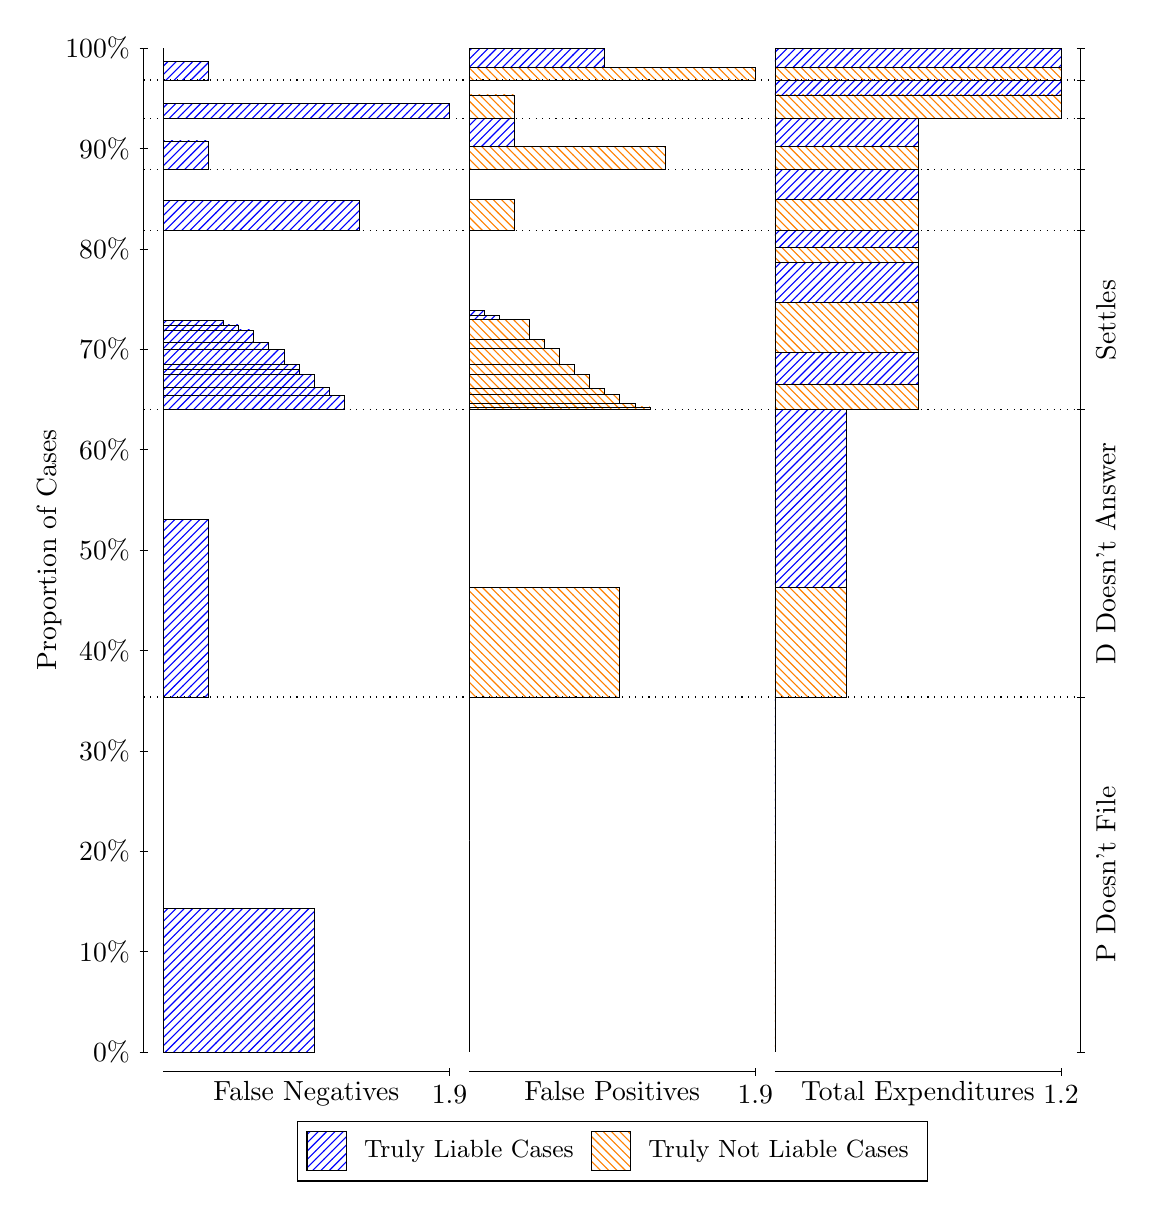
\begin{tikzpicture}
\draw[black, very thin] (1.5,1.75) -- (1.5,14.5);
\node[rotate=90, anchor=center] at (0.3, 8.125) {Proportion of Cases};
\draw[black, very thin] (1.45,1.75) -- (1.55,1.75);
\node[anchor=east] at (1.45, 1.75) {0\%};
\draw[black, very thin] (1.45,3.025) -- (1.55,3.025);
\node[anchor=east] at (1.45, 3.025) {10\%};
\draw[black, very thin] (1.45,4.3) -- (1.55,4.3);
\node[anchor=east] at (1.45, 4.3) {20\%};
\draw[black, very thin] (1.45,5.575) -- (1.55,5.575);
\node[anchor=east] at (1.45, 5.575) {30\%};
\draw[black, very thin] (1.45,6.85) -- (1.55,6.85);
\node[anchor=east] at (1.45, 6.85) {40\%};
\draw[black, very thin] (1.45,8.125) -- (1.55,8.125);
\node[anchor=east] at (1.45, 8.125) {50\%};
\draw[black, very thin] (1.45,9.4) -- (1.55,9.4);
\node[anchor=east] at (1.45, 9.4) {60\%};
\draw[black, very thin] (1.45,10.675) -- (1.55,10.675);
\node[anchor=east] at (1.45, 10.675) {70\%};
\draw[black, very thin] (1.45,11.95) -- (1.55,11.95);
\node[anchor=east] at (1.45, 11.95) {80\%};
\draw[black, very thin] (1.45,13.225) -- (1.55,13.225);
\node[anchor=east] at (1.45, 13.225) {90\%};
\draw[black, very thin] (1.45,14.5) -- (1.55,14.5);
\node[anchor=east] at (1.45, 14.5) {100\%};

\draw[black, very thin] (13.4,1.75) -- (13.4,14.5);
\draw[black, very thin] (13.35,1.75) -- (13.45,1.75);
\node[anchor=west] at (13.35, 1.75) {};
\draw[black, very thin] (13.35,6.2575) -- (13.45,6.2575);
\node[anchor=west] at (13.35, 6.2575) {};
\draw[black, very thin] (13.35,9.9071) -- (13.45,9.9071);
\node[anchor=west] at (13.35, 9.9071) {};
\draw[black, very thin] (13.35,12.184) -- (13.45,12.184);
\node[anchor=west] at (13.35, 12.184) {};
\draw[black, very thin] (13.35,12.962) -- (13.45,12.962);
\node[anchor=west] at (13.35, 12.962) {};
\draw[black, very thin] (13.35,13.61) -- (13.45,13.61);
\node[anchor=west] at (13.35, 13.61) {};
\draw[black, very thin] (13.35,14.094) -- (13.45,14.094);
\node[anchor=west] at (13.35, 14.094) {};
\draw[black, very thin] (13.35,14.5) -- (13.45,14.5);
\node[anchor=west] at (13.35, 14.5) {};

\draw[black, very thin, pattern color=blue, pattern=north east lines] (1.75,1.75) rectangle (3.6623,3.5729);
\draw[black, very thin, pattern color=orange, pattern=north west lines] (1.75,3.5729) rectangle (1.75,6.2575);
\draw[black, very thin, pattern color=blue, pattern=north east lines] (1.75,6.2575) rectangle (2.3237,8.511);
\draw[black, very thin, pattern color=orange, pattern=north west lines] (1.75,8.511) rectangle (1.75,9.9071);
\draw[black, very thin, pattern color=blue, pattern=north east lines] (1.75,9.9071) rectangle (4.0447,10.093);
\draw[black, very thin, pattern color=blue, pattern=north east lines] (1.75,10.093) rectangle (3.8535,10.188);
\draw[black, very thin, pattern color=blue, pattern=north east lines] (1.75,10.188) rectangle (3.6623,10.356);
\draw[black, very thin, pattern color=blue, pattern=north east lines] (1.75,10.356) rectangle (3.4711,10.421);
\draw[black, very thin, pattern color=blue, pattern=north east lines] (1.75,10.421) rectangle (3.4711,10.485);
\draw[black, very thin, pattern color=blue, pattern=north east lines] (1.75,10.485) rectangle (3.2798,10.668);
\draw[black, very thin, pattern color=blue, pattern=north east lines] (1.75,10.668) rectangle (3.0886,10.766);
\draw[black, very thin, pattern color=blue, pattern=north east lines] (1.75,10.766) rectangle (2.8974,10.92);
\draw[black, very thin, pattern color=blue, pattern=north east lines] (1.75,10.92) rectangle (2.7061,10.985);
\draw[black, very thin, pattern color=blue, pattern=north east lines] (1.75,10.985) rectangle (2.5149,11.037);
\draw[black, very thin, pattern color=orange, pattern=north west lines] (1.75,11.037) rectangle (1.75,12.184);
\draw[black, very thin, pattern color=blue, pattern=north east lines] (1.75,12.184) rectangle (4.236,12.564);
\draw[black, very thin, pattern color=orange, pattern=north west lines] (1.75,12.564) rectangle (1.75,12.962);
\draw[black, very thin, pattern color=blue, pattern=north east lines] (1.75,12.962) rectangle (2.3237,13.32);
\draw[black, very thin, pattern color=orange, pattern=north west lines] (1.75,13.32) rectangle (1.75,13.61);
\draw[black, very thin, pattern color=blue, pattern=north east lines] (1.75,13.61) rectangle (5.3833,13.799);
\draw[black, very thin, pattern color=orange, pattern=north west lines] (1.75,13.799) rectangle (1.75,14.094);
\draw[black, very thin, pattern color=blue, pattern=north east lines] (1.75,14.094) rectangle (2.3237,14.335);
\draw[black, very thin, pattern color=orange, pattern=north west lines] (1.75,14.335) rectangle (1.75,14.5);
\draw[black, very thin, pattern color=orange, pattern=north west lines] (5.6333,1.75) rectangle (5.6333,4.4346);
\draw[black, very thin, pattern color=blue, pattern=north east lines] (5.6333,4.4346) rectangle (5.6333,6.2575);
\draw[black, very thin, pattern color=orange, pattern=north west lines] (5.6333,6.2575) rectangle (7.5456,7.6535);
\draw[black, very thin, pattern color=blue, pattern=north east lines] (5.6333,7.6535) rectangle (5.6333,9.9071);
\draw[black, very thin, pattern color=orange, pattern=north west lines] (5.6333,9.9071) rectangle (7.9281,9.9421);
\draw[black, very thin, pattern color=orange, pattern=north west lines] (5.6333,9.9421) rectangle (7.7368,9.9886);
\draw[black, very thin, pattern color=orange, pattern=north west lines] (5.6333,9.9886) rectangle (7.5456,10.1);
\draw[black, very thin, pattern color=orange, pattern=north west lines] (5.6333,10.1) rectangle (7.3544,10.182);
\draw[black, very thin, pattern color=orange, pattern=north west lines] (5.6333,10.182) rectangle (7.1632,10.353);
\draw[black, very thin, pattern color=orange, pattern=north west lines] (5.6333,10.353) rectangle (6.9719,10.486);
\draw[black, very thin, pattern color=orange, pattern=north west lines] (5.6333,10.486) rectangle (6.7807,10.683);
\draw[black, very thin, pattern color=orange, pattern=north west lines] (5.6333,10.683) rectangle (6.5895,10.801);
\draw[black, very thin, pattern color=orange, pattern=north west lines] (5.6333,10.801) rectangle (6.3982,11.054);
\draw[black, very thin, pattern color=blue, pattern=north east lines] (5.6333,11.054) rectangle (6.0158,11.107);
\draw[black, very thin, pattern color=blue, pattern=north east lines] (5.6333,11.107) rectangle (5.8246,11.171);
\draw[black, very thin, pattern color=blue, pattern=north east lines] (5.6333,11.171) rectangle (5.6333,12.184);
\draw[black, very thin, pattern color=orange, pattern=north west lines] (5.6333,12.184) rectangle (6.207,12.582);
\draw[black, very thin, pattern color=blue, pattern=north east lines] (5.6333,12.582) rectangle (5.6333,12.962);
\draw[black, very thin, pattern color=orange, pattern=north west lines] (5.6333,12.962) rectangle (8.1193,13.252);
\draw[black, very thin, pattern color=blue, pattern=north east lines] (5.6333,13.252) rectangle (6.207,13.61);
\draw[black, very thin, pattern color=orange, pattern=north west lines] (5.6333,13.61) rectangle (6.207,13.904);
\draw[black, very thin, pattern color=blue, pattern=north east lines] (5.6333,13.904) rectangle (5.6333,14.094);
\draw[black, very thin, pattern color=orange, pattern=north west lines] (5.6333,14.094) rectangle (9.2667,14.258);
\draw[black, very thin, pattern color=blue, pattern=north east lines] (5.6333,14.258) rectangle (7.3544,14.5);
\draw[black, very thin, pattern color=orange, pattern=north west lines] (9.5167,1.75) rectangle (9.5167,4.4346);
\draw[black, very thin, pattern color=blue, pattern=north east lines] (9.5167,4.4346) rectangle (9.5167,6.2575);
\draw[black, very thin, pattern color=orange, pattern=north west lines] (9.5167,6.2575) rectangle (10.425,7.6535);
\draw[black, very thin, pattern color=blue, pattern=north east lines] (9.5167,7.6535) rectangle (10.425,9.9071);
\draw[black, very thin, pattern color=orange, pattern=north west lines] (9.5167,9.9071) rectangle (11.333,10.236);
\draw[black, very thin, pattern color=blue, pattern=north east lines] (9.5167,10.236) rectangle (11.333,10.639);
\draw[black, very thin, pattern color=orange, pattern=north west lines] (9.5167,10.639) rectangle (11.333,11.268);
\draw[black, very thin, pattern color=blue, pattern=north east lines] (9.5167,11.268) rectangle (11.333,11.782);
\draw[black, very thin, pattern color=orange, pattern=north west lines] (9.5167,11.782) rectangle (11.333,11.971);
\draw[black, very thin, pattern color=blue, pattern=north east lines] (9.5167,11.971) rectangle (11.333,12.184);
\draw[black, very thin, pattern color=orange, pattern=north west lines] (9.5167,12.184) rectangle (11.333,12.582);
\draw[black, very thin, pattern color=blue, pattern=north east lines] (9.5167,12.582) rectangle (11.333,12.962);
\draw[black, very thin, pattern color=orange, pattern=north west lines] (9.5167,12.962) rectangle (11.333,13.252);
\draw[black, very thin, pattern color=blue, pattern=north east lines] (9.5167,13.252) rectangle (11.333,13.61);
\draw[black, very thin, pattern color=orange, pattern=north west lines] (9.5167,13.61) rectangle (13.15,13.904);
\draw[black, very thin, pattern color=blue, pattern=north east lines] (9.5167,13.904) rectangle (13.15,14.094);
\draw[black, very thin, pattern color=orange, pattern=north west lines] (9.5167,14.094) rectangle (13.15,14.258);
\draw[black, very thin, pattern color=blue, pattern=north east lines] (9.5167,14.258) rectangle (13.15,14.5);
\draw[black, dotted] (1.5,6.2575) -- (13.4,6.2575);
\draw[black, dotted] (1.5,9.9071) -- (13.4,9.9071);
\draw[black, dotted] (1.5,12.184) -- (13.4,12.184);
\draw[black, dotted] (1.5,12.962) -- (13.4,12.962);
\draw[black, dotted] (1.5,13.61) -- (13.4,13.61);
\draw[black, dotted] (1.5,14.094) -- (13.4,14.094);
\draw[black, very thin] (1.75,1.5) -- (5.3833,1.5);
\node[anchor=north] at (3.5667, 1.5) {False Negatives};
\draw[black, very thin] (5.3833,1.45) -- (5.3833,1.55);
\node[anchor=north] at (5.3833, 1.45) {1.9};

\draw[black, very thin] (5.6333,1.5) -- (9.2667,1.5);
\node[anchor=north] at (7.45, 1.5) {False Positives};
\draw[black, very thin] (9.2667,1.45) -- (9.2667,1.55);
\node[anchor=north] at (9.2667, 1.45) {1.9};

\draw[black, very thin] (9.5167,1.5) -- (13.15,1.5);
\node[anchor=north] at (11.333, 1.5) {Total Expenditures};
\draw[black, very thin] (13.15,1.45) -- (13.15,1.55);
\node[anchor=north] at (13.15, 1.45) {1.2};

\node[black, centered, rotate=90] at (13.72, 4.0037) {P Doesn't File};
\node[black, centered, rotate=90] at (13.72, 8.0823) {D Doesn't Answer};
\node[black, centered, rotate=90] at (13.72, 11.046) {Settles};





\draw (7.449999999999999,1.5) node[draw=none] (baseCoordinate) {};
\begin{scope}[align=center]
        \matrix[scale=0.5, draw=black, below=0.5cm of baseCoordinate, nodes={draw}, column sep=0.1cm]{
            \node[rectangle, draw, minimum width=0.5cm, minimum height=0.5cm, pattern=north east lines, pattern color=blue] {}; &
            \node[draw=none, font=\small] (B) {Truly Liable Cases}; &
            \node[rectangle, draw, minimum width=0.5cm, minimum height=0.5cm, pattern=north west lines, pattern color=orange] {}; &
            \node[draw=none, font=\small] (B) {Truly Not Liable Cases}; \\
            };
\end{scope}

\end{tikzpicture}
\end{document}